\subsection{A7 School Improvement Process Criterion}

The school leadership facilitates school improvement which (a) is driven by plans of action that will enhance quality learning for all students, (b) has school community support and involvement, (c) effectively guides the work of the school, and (d) provides for accountability through monitoring of the schoolwide action plan.

\subsubsection{Broad-based and Collaborative}

\indicator{The school’s planning process is broad-based, collaborative, and has commitment of the stakeholders, including the staff, students, and parents.}

\prompt{Comment on the effectiveness of the school planning process to ensure that it is broad-based, collaborative, and fosters the commitment of the stakeholders, including the staff, students, and parents.}

\begin{findings}
CMIS has several plans and processes in place that are broad-based, collaborative, and have commitment of the stakeholders, including the staff, students, and parents.

During the Curriculum Review Cycle CMIS work together to vet materials and resources to ensure standards alignment, instructional relevancy and high quality of material.

The\href{https://docs.google.com/a/cmis.ac.th/document/d/1iW_tWIwRlWU2p0oIOvd3usDsxj9qYDt_2ROwNPBTHSc/edit?usp=sharing}{ Teacher Leadership Team}  and administrative team collaborate on ways to support PK-12 teachers with: instructional best practices, curriculum planning, assessment design, and data analysis. 

UbD curriculum design and scope/sequence blueprints are utilized by all teachers and facilitated by our teacher leadership team. These team plans foster shared responsibility, and instructional accountability, and are directly related to our SLOs which support student learning in a global environment. 

The CMIS \href{http://blogs.cmis.ac.th/campus/}{Campus Development Team} works with students, teachers and parents to keep them updated and aware of campus restoration and development progress.

The  PTG monthly meeting fosters communication between the teachers, parents and the school. Topics for discussion are \href{https://docs.google.com/a/cmis.ac.th/document/d/1kiwakkg8eKdtEexCxVNx-m1CfC3VqxhukDy8WXDPGKY/edit?usp=sharing}{parent generated} and based on parent feedback. The school management and parent translators are always present for support.

\minor{So what...}
The findings indicate that CMIS addresses this indicator by using broad-based, collaborative opportunities to demonstrate commitment of the stakeholders, including the staff, students, and parents. Processes and protocols should be developed to include more example of collaborating with students.
\end{findings}

\subsubsection{School Plan Correlated to Student Learning}

\indicator{The school’s action plan is directly correlated to the analysis of student achievement data about the critical learner needs, schoolwide learner outcomes, and academic standards.}

\prompt{How does the school ensure that the analysis of student achievement about the critical learner needs, schoolwide learner outcomes, and academic standards impacts the development, implementation, and monitoring of the plan?}

\begin{findings}
The CMIS Action Plan is correlated to the analysis of student achievement data based on critical learner needs, schoolwide learner outcomes, and academic standards.
Increasing student achievement is always at the center of CMIS efforts. The Mission and Vision was rewritten in 2015 to be aligned with the new SLOs. The process involved the review of the community profile, student achievement, and the identification of CMIS critical learner needs in a global environment.
Using research-based models, CMIS adopted academic standards that are at the center of all planning. CMIS Leadership and Teaching Staff have taken measures to evaluate program progress and implementation. The use of department meetings to discuss coherence between instruction, planning, and standards takes place regularly. The CMIS Teaching Staff use and modify, if necessary, Scope and Sequence Blueprints to identify instructional gaps. Teacher created UbD units also ask the designer to address primary and secondary standards that are aligned with the instructional goal. Feedback from the Teacher Leadership Team is provided to the teachers about the alignment of the unit areas (i.e. standards, essential questions, skills, knowledge, learning activities, and assessment). 

\minor{So what...}

Though the CMIS Teaching Staff have made great strides in maintaining and monitoring the academic standards, more work could be devoted to providing time and resources for a deeper analysis of the standards. Identifying the deep structures and pedagogical shifts in instruction also require attention in planning, instruction, and assessment.  

The first Future Focus Area directly addresses the challenge of analyzing data to make informed decisions about critical learner needs, schoolwide learner outcomes, and academic standards. 
\end{findings}

\subsubsection{Systems Alignment}

\indicator{Within the school there is evidence of systems alignment in areas such as professional goals, teacher evaluation, and strategic planning for the purpose of ongoing school improvement.}

\prompt{What evidence supports the systems alignment in areas such as professional goals, teacher evaluation, and strategic planning for the purpose of ongoing school improvement?}

\begin{findings}
CMIS incorporates several means to ensure systems alignment in areas such as professional goals, teacher evaluation, and strategic planning for the purpose of ongoing school improvement.

The CMIS \href{https://docs.google.com/a/cmis.ac.th/presentation/d/1sWhr1U3qZIGEu2aQdWOl0OQ5Rkd8iRGWmUlszEJLz2o/edit?usp=sharing}{Student Success Team} consists of the health officer, counselors, and the learning support teachers. They meet regularly to review and strategically plan ways to increase student academic achievement, physical safety, and emotional wellbeing. If teachers have student concerns they are encouraged to reach out to the Student Success Team led by the Student Service Coordinator. There is a \href{https://docs.google.com/a/cmis.ac.th/forms/d/e/1FAIpQLScVtFtaEXarGOjwsiJyGdbLAMbeNzG9m44i1fWXFLbtMKZcUg/viewform}{Student Service Request Form} available on the teacher dashboard section of the CMIS website.This form activates immediate support from the team to meet with the teacher and create a plan of action.

In 2014 all teachers were trained and have since participated in the year long, research based \href{https://drive.google.com/a/cmis.ac.th/file/d/0B71_pYxcTLo-OExlV0Y5UVFBNVU/view?usp=sharing}{Datawise Process}. Data Wise a school wide improvement process that organizes and brings coherence to the work of school improvement.  It is a specific and strategic process that facilitates intentional thinking and utilizing a disciplined way of looking at student data as a collaborative group. Datawise helps the CMIS Teaching Staff learn how to analyze data in a manner that contributes to improved instruction and increased student learning. CMIS creates an annual \href{https://docs.google.com/document/d/1TmnCp5qZiZAUMnUmaU32PBn2UGvCMVtFO8r5OsxwNo4/edit}{Datawise Plan} that identifies learner centered problems (LCP) at each department level and includes instructional strategies to address them as well as assessment practices to evaluate student progress.

The modified, research based CMIS teacher \href{https://docs.google.com/document/d/15_5X5QtixmWVheEUBVO9N1aislsLDm_ZW4-4g4YQ7F4/edit?usp=sharing}{evaluation process} focuses on the teacher reviewing observational data to identify student learning, increase student learning opportunities and promote desired student global competencies. The model encourages CMIS teachers to reflect deeply on their practice and align it to student achievement through a common framework and vocabulary. It helps teachers determine the focus of their professional development based on what is actually occurring (or not occurring) in their classroom, and set meaningful goals for increased student achievement. 

Since 2015, all CMIS teachers have been trained and have participated in the \href{https://drive.google.com/a/cmis.ac.th/file/d/0B0TYmzaZNi3fUzVFUEdzTURtakk/view?usp=sharing}{Instructional Rounds} protocol. Instructional Rounds are structured observations between teachers. During the Instructional Round period, student data is collected which focuses on teacher deliberative practice and student achievement. These opportunities support teachers to make professional goals, provide self-reflection, and align their teaching with the school focus of ongoing school improvement See sections entitled: Congruence and Collaborative Work for more information on instructional rounds. 

\minor{So what...}

Continue to monitor and maintain the instructional rounds process, datawise, and the teacher evaluation instrument to create professional development opportunities based on deliberative practice stemming from those processes.
\end{findings}

\subsubsection{Correlation between All Resources, Schoolwide Learner Outcomes, and Action Plan}

\indicator{There is correlation between allocation of time/fiscal/personnel/material resources and the implementation, monitoring, and accomplishing of the schoolwide action plan.}

\prompt{Examine and evaluate the degree to which the allocation of time/fiscal/personnel/ material resources support the implementation, monitoring, and accomplishment of the schoolwide action plan.}

\begin{findings}
CMIS allocates time, fiscal, material, and personnel resources to the accomplishment, implementation, and monitoring of the schoolwide action plan. 

Implementation of the schoolwide action plan is in its early stages, but progress has been made in all Future Focus Areas. A prototype of the Data Sandbox has been developed. Project benchmarks have been created and staff have been allocated for this project. The same is true for the CMIS Marketing focus. A Marketing Committee has been created and have already attended a training on effective international school marketing strategies. Of course, to address the Staffing Focus Area, improving the interviewing, hiring, and orientation of new staff is always an ongoing process and has been strengthened for this year’s recruitment process.  The division principals, teachers, and the school executive team are involved in this process. Finally, to address the Funding Focus Area, an alumni coordinator continues to work at developing funding sources from the CMIS Alumni base and a public relations and fundraising committee continues to monitor and develop new funding sources. Each of these Focus Areas will continue to be monitored and evaluated for program success. 

\minor{So what...}
CMIS has developed four sound and strategic Focus Areas for improvement. Please see CMIS School Wide Action Plan for more information. 
\end{findings}


{\centering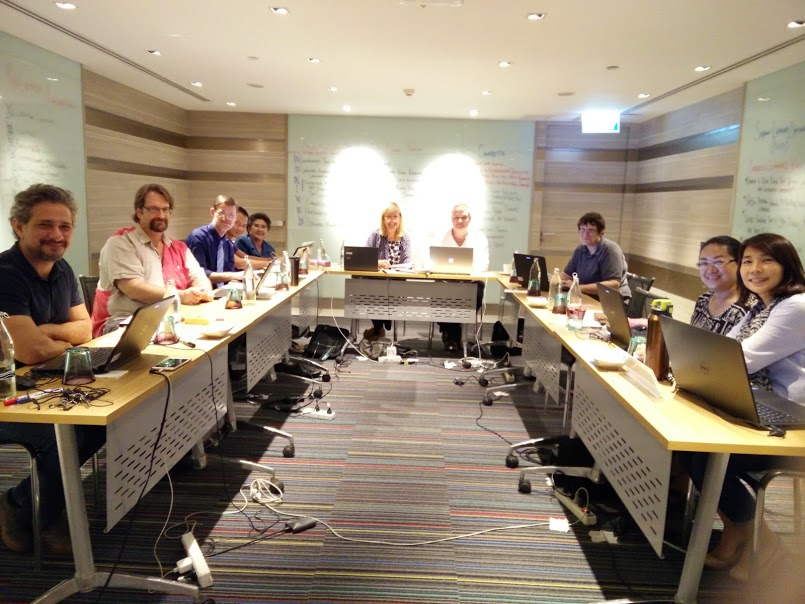
\includegraphics[width=\textwidth]{chapter4_A7.JPG}}


\subsection{Conclusions}
\prompt{Comment on the degree to which this criterion is being addressed.}

\begin{findings}
The finding suggest that this criterion is being addressed to a high degree as CMIS Leadership have created actionable, realistic, and measureable goals to ensure that the CMIS Action Plan is addressed and implemented. 

\minor{Maintain and Monitor}
\begin{itemize}
\item Datawise process in all grade levels
\item CMIS adopted standards analysis, implementation, and instructional accountability
\item Instructional Rounds peer observation protocol 
\item Research based Teacher Evaluation protocol 
\item Teacher Leadership Team participation and input 
\item CMIS Campus Development Team participation and input
\item UbD unit creation and implementation
\item Student Success Team and Student Service Coordinator roles
\end{itemize}
 

\minor{Continue to Improve}
\begin{itemize}
\item Providing student leadership opportunities in established committees
\item Marketing strategies
\item Public relations strategies 
\item Alumni connection strategies
\end{itemize}
 
\end{findings}
